\documentclass[11pt,a4paper]{article}

%-------------------------------------
%            Informations Générales
%-------------------------------------

%\NeedsTeXFormat{LaTeX2e}[2009/09/24]
%\ProvidesPackage{style}[2009/09/24 Extension personnelle, V1.0]

%-------------------------------------
% 						extensions
%-------------------------------------
\usepackage[T1]{fontenc} 
\usepackage[utf8]{inputenc}
\usepackage[francais]{babel}
\usepackage{url}
\usepackage{etex}
\usepackage{enumitem}
\usepackage{multicol}
\usepackage{bbm}
\usepackage{amsmath,amsthm,amssymb}
\usepackage[official]{eurosym}
%\usepackage{pifont}
\usepackage[left=1cm, right=1cm, top=1.5cm, bottom=1.5cm]{geometry}
\usepackage{exercise}
\usepackage{graphics}
\usepackage{array,multirow,makecell}
\usepackage{verbatim}
\usepackage[dvipsnames,table]{pstricks}
\usepackage{pstricks-add,pst-plot,pst-text,pst-tree,pst-eps,pst-fill,pst-node,pst-math,pst-blur,pst-func}
\usepackage{pgf,tikz}
\usepackage{tipfr}
\usepackage{thmbox}
\usepackage{calc}
\usepackage{ifthen}
\usepackage{pdfpages}
\usepackage{colortbl}
%\usepackage{sagetex}
\usetikzlibrary{arrows,patterns}
%\input tabvar
\usepackage{tkz-tab}
\usepackage{listings}
\usepackage[np]{numprint}
%\usepackage{tabularx}
\usepackage{fancybox,fancyhdr}
\usepackage{thmtools}
\usepackage{bclogo}
\usepackage{lastpage}

%------------------------------------- 
%        		Abréviations personnelles
%-------------------------------------
\newcommand{\Cc}{\textbf{Conclusion: }}
\newcommand{\DNS}{\textbf{Devoir Non Surveillé}}
\newcommand{\DS}{\textbf{Devoir Surveillé}}
\newcommand\fpsd{une fonction polynôme du second degré~}
\newcommand{\N}{\mathbb{N} } % Raccourci pour l'ensemble des entiers naturels
\newcommand{\R}{\mathbb{R}} % Raccourci pour l'ensemble des réels
\newcommand{\Z}{\mathbb{Z}} % Raccourci pour l'ensemble des entiers relatifs
%\newcommand{\N}{\mathbb{N}} % Raccourci pour l'ensemble des réels

%----------------------------------------------------------------------------------------------- 
% 							Commandes mathématiques
%-----------------------------------------------------------------------------------------------
\renewcommand{\vec}[1]{\overrightarrow{#1}}	% Raccourci pour vecteurs
\newcommand{\inv}[1]{\dfrac{1}{#1}} % Raccourci pour l'inverse des réels
\newcommand{\e}{\text{e}}
\newcommand*{\E}{\ensuremath{\mathrm{e}}}
\newcommand{\lnx}{\ln(x)}

%----------------------------------------------------------------------------------------------- 
% 							Commandes Tableaux
%-----------------------------------------------------------------------------------------------
\setcellgapes{3pt}
\makegapedcells\newcolumntype{R}[1]{>{\raggedleft\arraybackslash}b{#1}}
\newcolumntype{L}[1]{>{\raggedright\arraybackslash}b{#1}}
\newcolumntype{C}[1]{>{\centering\arraybackslash}b{#1}}

%----------------------------------------------------------------------------------------------- 
% 							Commandes Listes
%-----------------------------------------------------------------------------------------------
% Redéfinition du premier niveau
\renewcommand{\theenumi}{\arabic{enumi}}
\renewcommand{\labelenumi}{\textbf{\theenumi}}
% Redéfinition du deuxième niveau
\renewcommand{\theenumii}{\alph{enumii}}
\renewcommand{\labelenumii}{\textbf{\theenumii}}

%-----------------------------------------------------------------------------------------------
%							 		Environnement - Macros
%-----------------------------------------------------------------------------------------------
\setlength{\columnsep}{20pt}
\setlength{\columnseprule}{0.5pt}
\renewcommand{\thesection}{\arabic{section}}
%\renewcommand{\thesection}{\arabic{section}}
%La numérotation des section repart à 0 lorsque l'on change de partie
%\makeatletter\@addtoreset{section}{chapter}\makeatother
\makeatletter\@addtoreset{subsection}{section}\makeatother
%\renewcommand{\thechapter}{\arabic{chapter}}
%\renewcommand{\thesection}{\arabic{section}}
\renewcommand{\thesubsection}{\arabic{subsection}}
%Modifier la section dans son positionnement, sa forme, couleur,...
%\makeatletter
%\renewcommand\section{\@startsection {section}{1}{\z@}%
%                                   {-1.5ex \@plus -0.5ex \@minus -.2ex}%
 %                                  {1.8ex \@plus .2ex}%
  %                                 {\raggedleft\normalfont\color{gray}\large\bfseries}}
%\makeatother
\newenvironment{maliste}%
{ \begin{list}%
	{$\bullet$}%
	{\setlength{\labelwidth}{30pt}%
	 \setlength{\leftmargin}{35pt}%
	 \setlength{\itemsep}{\parsep}}}%
{ \end{list} }


%------------------------------------------------------------------------------------------------
% Paramétrage du langage TI pour la reconnaissance des mots clé utilisés
% A compléter avec les fonctions du catalogue de texas.
%------------------------------------------------------------------------------------------------
\lstdefinelanguage{TI}{%
       morekeywords={%
        %%% CONTROLE.
          If, Then, Else, For, While, Repeat, End, Pause, Lbl, Goto, IS>, DS<, Menu, prgm, Return, Stop, EffVar, GraphStyle,
        %%% ENTREES & SORTIES
          Input, Prompt, Disp, AffGraph, AffTable, Output, codeTouch, EffEcr, EffTable, CaptVar,
        %%% CATALOG
         NbrAléat,
        %%% FONCTIONS NUMERIQUES
          cos, sin, tan, acos, asin, atan,
        %%% CONSTANTES
          pi,
      },
      sensitive=true,
      morecomment=[l]{\#},
      morestring=[b]',
    }


%---------------------------------------------------------------------------------------- 
% 									Environnement NSI
%----------------------------------------------------------------------------------------

\newenvironment{NSI}[2]
{
	\noindent
	\setlength{\fboxsep}{0cm}\setlength{\fboxrule}{0pt}\framebox[19cm]{
		\setlength{\fboxsep}{0.25cm}\setlength{\fboxrule}{1pt}
		\Huge{\textbf{#1:}}
		\hspace{0.5cm}{\huge{#2}}\hfill
	}
	{\newline \rule[0cm]{\linewidth}{0.05em}}
}

%---------------------------------------------------------------------------------------- 
% 									Environnement de cours
%----------------------------------------------------------------------------------------
\newcounter{nbCrs}
%\setcounter{nbCrs}{1}

\newenvironment{headCrs}[1]
{
	\addtocounter{nbCrs}{1}
	\noindent
	\setlength{\fboxsep}{0cm}\setlength{\fboxrule}{0pt}\framebox[19cm]{
		\setlength{\fboxsep}{0.25cm}\setlength{\fboxrule}{1pt}
		\Ovalbox{\Huge{\textbf{\thenbCrs}}}
		\hspace{0cm plus 1fill}{\huge{\textbf{#1}}}
	}
	{\newline \rule[-0.3cm]{\linewidth}{0.05em}}
}



%-----------------------------------------------------------------------------------------------
% 								Environnement d'Activité
%-----------------------------------------------------------------------------------------------
\newcounter{nbAct}
%\setcounter{nbAct}{1}

\newenvironment{headAct}[1]
{
	\setlength{\fboxsep}{-0.5cm}\setlength{\fboxrule}{0pt} 
	\ifthenelse{\equal{#1}{Activité}}
		{
			\addtocounter{nbAct}{1}
			\noindent
			\framebox[19cm]{
				\begin{Huge}
					$\rhd$ %\hspace{\stretch{1}} 
					\textbf{#1~\thenbAct}
					\hspace{\stretch{1}} %$\bigcirc$
				\end{Huge}			  
			}
		}
		{
			\noindent
			\framebox[19cm]{
				\begin{Huge}
					$\bigcirc$ \hspace{\stretch{1}} 
					\textbf{#1~\thenbAct}
					\hspace{\stretch{1}} $\bigcirc$
				\end{Huge}				  
			}
		}
}
{\newline \rule{\linewidth}{1pt} \medskip}

%-----------------------------------------------------------------------------------------------
% 								Environnement d'AP
%-----------------------------------------------------------------------------------------------
\newcounter{nbAP}

\newenvironment{headAP}[1]
{
	\setlength{\fboxsep}{-0.5cm}\setlength{\fboxrule}{0pt} 
	\ifthenelse{\equal{#1}{Accompagnement Personnalisé}}
		{
			\addtocounter{nbAP}{1}
			\framebox[18cm]{
				\begin{Huge}
					$\square$ \hspace{\stretch{1}} 
					\textbf{#1~\thenbAP}
					\hspace{\stretch{1}} $\square$
				\end{Huge}				  
			}
		}
		{
			\framebox[18cm]{
				\begin{Huge}
					$\square$ \hspace{\stretch{1}} 
					\textbf{#1~\thenbAP}
					\hspace{\stretch{1}} $\square$
				\end{Huge}				  
			}
		}
}
{\newline \rule{\linewidth}{1pt}}

%------------------------------------- 
% 				Environnement Exercices
%-------------------------------------
\newcounter{nbEx}
%\setcounter{nbAct}{1}

\newenvironment{headEx}[1]
{
	\setlength{\fboxsep}{-0.5cm}\setlength{\fboxrule}{0pt} 
	\ifthenelse{\equal{#1}{Exercices}}
		{
			\addtocounter{nbEx}{1}
			\framebox[18cm]{
				\begin{Huge}
					\textbf{#1}
					\hspace{\stretch{1}} \textbf{\thenbEx}
				\end{Huge}				  
			}
		}
		{
			\framebox[18cm]{
				\begin{Huge}
					\textbf{#1}
					\hspace{\stretch{1}} \textbf{\thenbEx}
				\end{Huge}				  
			}
		}
}
{\newline \rule{\linewidth}{1pt}}

%------------------------------------- 
% 				Environnement TP Info
%-------------------------------------
\newcounter{nbTP}

\newenvironment{headTP}[1]
{
	\setlength{\fboxsep}{-0.5cm}\setlength{\fboxrule}{0pt} 
	\ifthenelse{\equal{#1}{TP}}
		{
			\addtocounter{nbTP}{1}
			\framebox[18cm]{
				\begin{Huge}
					\textbf{#1}
					\hspace{\stretch{1}} \textbf{\thenbTP}
				\end{Huge}				  
			}
		}
		{
			\framebox[18cm]{
				\begin{Huge}
					\textbf{#1}
					\hspace{\stretch{1}} \textbf{\thenbTP}
				\end{Huge}				  
			}
		}
}
{\newline \rule{\linewidth}{1pt}}


%------------------------------------- 
% 				Environnement DNS
%-------------------------------------
\newcounter{nbDNS}
%\setcounter{nbDNS}{1}

\newenvironment{headDNS}[4]	%{DNS}{date}{sujet}{classe}
{
	\setlength{\fboxsep}{0.25cm}\setlength{\fboxrule}{0pt} 
	\ifthenelse{\equal{#1}{DNS}}
		{
			\addtocounter{nbDNS}{1}
			\noindent
			\framebox[18.5cm]{
					\LARGE{\DNS} \textbf{~\thenbDNS} \hspace{\stretch{1}} \large{#2}
			}
			\newline
			\framebox[18.5cm]{
					\makebox[2\width]{\small{#3}} \hspace{\stretch{1}} \makebox[5\width]{\large{#4}}
			}
		}
		{
			%\addtocounter{nbDNS}{1}			
			\noindent
			\framebox[18.5cm]{
					\LARGE{ #1 } \textbf{~\thenbDNS} \hspace{\stretch{1}} \large{#2}
			}
			\newline
			\framebox[18.5cm]{
					\makebox[2\width]{\small{#3}} \hspace{\stretch{1}} \makebox[5\width]{\large{#4}}
			}
		}
}
{\newline \rule{\linewidth}{1pt}}

%------------------------------------- 
% 				Environnement DS
%-------------------------------------
\newcounter{nbDS}
%\setcounter{nbDS}{1}

\newenvironment{headDS}[4]	%{DS}{date}{sujet}{classe}
{
	\setlength{\fboxsep}{0.25cm}\setlength{\fboxrule}{0pt} 
	\ifthenelse{\equal{#1}{DS}}
		{
			\addtocounter{nbDS}{1}
			\noindent
			\framebox[18.5cm]{
					\LARGE{\DS} \textbf{~\thenbDS} \hspace{\stretch{1}} \large{#2}
			}
			\newline
			\framebox[18.5cm]{
					\makebox[2\width]{\small{#3}} \hspace{\stretch{1}} 	\makebox[2\width]{\large{#4}}
			}
		}
		{
			\noindent
			\framebox[18.5cm]{
					\Large{ #1 } \textbf{~\thenbDS} \hspace{\stretch{1}} \large{#2}
			}
			\newline
			\framebox[18.5cm]{
					\makebox[2\width]{\small{#3}} \hspace{\stretch{1}}\hfill \makebox[5\width]{\large{#4}}
			}
		}
}
{\newline \rule{\linewidth}{1pt}\bigskip}

%------------------------------------- 
% 				Environnement de TEST
%-------------------------------------
\newcounter{nbTEST}
%\setcounter{nbTEST}{1}

\newenvironment{headTEST}[2]	%{Test}{classe}
{
	\setlength{\fboxsep}{0.25cm}\setlength{\fboxrule}{0pt} 
	\ifthenelse{\equal{#1}{TEST}}
		{
			\addtocounter{nbTEST}{1}
			\noindent
			\framebox[18.5cm]{
					\makebox[4cm]{\LARGE{ #1 } \textbf{~\thenbTEST}} \hspace{\stretch{1}} \makebox[8cm][l]{\LARGE{Nom:}}
			}
			\newline
			\framebox[18.5cm]{
					\makebox[4cm]{\large{#2}} \hspace{\stretch{1}} \makebox[8cm][l]{\LARGE{Prénom:}}
			}
		}
		{
			\noindent
			\framebox[18.5cm]{
					\Large{ #1 } \textbf{~\thenbTEST} \hspace{\stretch{1}} \makebox[10cm]{Corrigé}
			}
			\newline
			\framebox[18.5cm]{
					\makebox[6cm]{\small{#2}}
			}
		}
}
{\newline \rule{\linewidth}{1pt}}

%------------------------------------- 
% 				Environnement de ACQUIS
%-------------------------------------
\newcounter{nbACQUIS}
%\setcounter{nbTEST}{1}

\newenvironment{headACQUIS}[2]	%{Test}{classe}
{
	\setlength{\fboxsep}{0.25cm}\setlength{\fboxrule}{0pt} 
	\ifthenelse{\equal{#1}{ACQUIS}}
		{
			\addtocounter{nbACQUIS}{1}
			\noindent
			\framebox[18.5cm]{
					\makebox[4cm]{\LARGE{ #1 } \textbf{~\thenbACQUIS}} \hspace{\stretch{1}} \makebox[8cm][l]{\LARGE{Nom:}}
			}
			\newline
			\framebox[18.5cm]{
					\makebox[4cm]{\large{#2}} \hspace{\stretch{1}} \makebox[8cm][l]{\LARGE{Prénom:}}
			}
		}
		{
			\noindent
			\framebox[18.5cm]{
					\Large{ #1 } \textbf{~\thenbACQUIS} \hspace{\stretch{1}} \makebox[10cm]{Corrigé}
			}
			\newline
			\framebox[18.5cm]{
					\makebox[6cm]{\small{#2}}
			}
		}
}
{\newline \rule{\linewidth}{1pt}}

%------------------------------------- 
% 				Environnement de QCM
%-------------------------------------
\newcounter{nbQCM}
%\setcounter{nbQCM}{1}

\newenvironment{headQCM}[2]	%{QCM}{classe}
{
	\setlength{\fboxsep}{0.25cm}\setlength{\fboxrule}{0pt} 
	\ifthenelse{\equal{#1}{QCM}}
		{
			\addtocounter{nbQCM}{1}
			\noindent
			\framebox[18.5cm]{
					\makebox[4cm]{\LARGE{ #1 } \textbf{~\thenbQCM}} \hspace{\stretch{1}} \makebox[8cm][l]{\LARGE{Nom:}}
			}
			\newline
			\framebox[18.5cm]{
					\makebox[4cm]{\large{#2}} \hspace{\stretch{1}} \makebox[8cm][l]{\LARGE{Prénom:}}
			}
		}
		{
			\noindent
			\framebox[18.5cm]{
					\Large{ #1 } \textbf{~\thenbQCM} \hspace{\stretch{1}} \makebox[10cm]{Corrigé}
			}
			\newline
			\framebox[18.5cm]{
					\makebox[6cm]{\small{#2}}
			}
		}
}
{\newline \rule{\linewidth}{1pt}}



%------------------------------------- 
% 				Environnement de DSSC
%-------------------------------------
\newcounter{nbDSSC}
%\setcounter{nbQCM}{1}

\newenvironment{headDSSC}[2]	%{DSSC}{classe}
{
	\setlength{\fboxsep}{0.25cm}\setlength{\fboxrule}{0pt} 
	\ifthenelse{\equal{#1}{DS}}
		{
			\addtocounter{nbDSSC}{1}
			\noindent
			\framebox[18.5cm]{
					\makebox[4cm]{\LARGE{ #1 } \textbf{~\thenbDSSC}} \hspace{\stretch{1}} \makebox[8cm][l]{\LARGE{Nom:}}
			}
			\newline
			\framebox[18.5cm]{
					\makebox[4cm]{\large{#2}} \hspace{\stretch{1}} \makebox[8cm][l]{\LARGE{Prénom:}}
			}
		}
		{
			\noindent
			\framebox[18.5cm]{
					\Large{ #1 } \textbf{~\thenbDSSC} \hspace{\stretch{1}} \makebox[10cm]{Corrigé}
			}
			\newline
			\framebox[18.5cm]{
					\makebox[6cm]{\small{#2}}
			}
		}
}
{\newline \rule{\linewidth}{1pt}}

%-------------------------------------
% 					Table des matières
%-------------------------------------

\renewcommand{\contentsname}{Sommaire} 


%-------------------------------------
% 					Fin du package
%-------------------------------------

%\endinput


\newcounter{num}
\newcounter{rem}
\setcounter{num}{0}
\setcounter{rem}{0}
\renewcommand{\arraystretch}{1.25}
%\setlength{\tabcolsep}{0.4cm}
\setlength{\parindent}{0cm}

\newcommand{\Frac}[2]{\displaystyle{\frac{#1}{#2}}}

\usepackage{hyperref}
\newcommand{\esp}{\hspace{0.5cm}}
\newcommand{\espp}{\hspace{1cm}}
\newcommand{\esppp}{\hspace{1.5cm}}
\renewcommand{\arraystretch}{1.5}

\hypersetup{
    colorlinks =false,
    linkcolor=blue,
   linkbordercolor = 1 0 0
}
\newcounter{numexo}
\setcellgapes{1pt}


\begin{document}

\begin{NSI}
{Exercice}{Recherche par dichotomie}
\end{NSI}

On redonne l'algorithme de recheche par dichotomie en langage python.\medskip

\hspace{1cm}\fbox{\begin{minipage}{10cm}
$a=0$\\
$b=\text{len}(t)-1$\\
\textbf{while} $a <= b$: 

\esp$m=(a+b)//2 $

\esp\textbf{if}$v<t[m]$:

\espp$b=m-1$

\esp\textbf{elif} $v>t[m]$:

\espp$a=m+1$

\esp\textbf{sinon} return $m$\\
return $-1$  
\end{minipage}}
\medskip

La valeur $-1$ est retournée lorsque le nombre n'est pas présent dans le tableau. On pourrait choisir une autre valeur ou même une chaine de caractère!


\addtocounter{numexo}{1}
\subsection*{\Large Exercice \thenumexo}
Max et Lilly joue à devine nombre. Max pense à un nombre entier compris entre 1 et 100 et Lilly doit le trouver. À chaque nombre proposé par Lilly, Max lui dit s'il est plus petit ou plus grand. 

Si Lilly applique la recherche par dichotomie, en combien d'essais au maximum peut-elle trouver le nombre de Max?


\addtocounter{numexo}{1}
\subsection*{\Large Exercice \thenumexo}
Soit T un tableau trié tel que: $T=[8, 8, 17, 21, 23, 27, 28, 45, 57, 71, 77, 84, 88, 95, 97]$.
\begin{enumerate}
\item On veut vérifier la présence du nombre $23$ dans le tableau.
\begin{enumerate}
\item Retracer toutes les étapes de l'algorithme de recherche par dichotomie.
\item Combien d'itérations ont été nécessaires?
\end{enumerate}
\item Faire de même avec le nombre $88$.
\item Faire de même avec le nombre $75$.
\end{enumerate}


\addtocounter{numexo}{1}
\subsection*{\Large Exercice \thenumexo}
\begin{enumerate}
\item Créer un tableau $T$ de valeurs choisies aléatoirement entre 1 et 1000.
\item Trier ce tableau avec une des fonctions de tri de python.
\item Écrire l'algorithme de recherche par dichotomie en langage python.
\item Tester votre programme avec la recherche de différentes valeurs du tableau et des valeurs qui ne sont pas dans le tableau.
\end{enumerate}

\newpage

\setcounter{numexo}{0}
\addtocounter{numexo}{1}
\subsection*{\Large Exercice \thenumexo}
La situation nécessitant le maximum d'essais est celle qui conduit à avoir $a=b$. On peut chercher le nombre d'itérations pour avoir $a=b=1$. Rassemblons les valeurs dans un tableau:\medskip

\begin{tabular}{|C{2.5cm}*{8}{|C{1cm}}|}
    \hline
    itérations& & $1$ & $2$ & $3$ & $4$ & $5$ & $6$ & $7$ \\
    \hline
    $m=(a+b)//2$&&$50$&$25$&$12$&$6$&$3$&$1$&$1$\\
    \hline
    $a$&$1$&$1$&$1$&$1$&$1$&$1$&$1$&$1$\\
    \hline
    $b$&$100$&$49$&$24$&$11$&$5$&$2$&$1$&$0$\\
    \hline
\end{tabular}\medskip

Ce tableau montre qu'au maximum 7 itérations seront nécessaires pour trouver le nombre pensé par Max.

\addtocounter{numexo}{1}
\subsection*{\Large Exercice \thenumexo}
Soit T un tableau trié tel que: $T=[8, 8, 17, 21, 23, 27, 28, 45, 57, 71, 77, 84, 88, 95, 97]$.
\begin{enumerate}
\item On veut vérifier la présence du nombre $23$ dans le tableau.
\begin{enumerate}
\item Le tableau trié contient $15$ valeurs donc $a=0$ et $b=14$.\medskip

\begin{tabular}{|C{2.5cm}*{5}{|C{1cm}}|}\hline
itérations &&$1$&$2$&$3$&$4$\\\hline
$m=(a+b)//2$&&$7$&$3$&$5$&$4$\\\hline
$T[m]$&&$45$&$21$&$27$&$23$\\\hline
$a$&$0$&$0$&$4$&$4$&\\\hline
$b$&$14$&$6$&$6$&$5$&\\\hline
\end{tabular}\medskip


\item 4 itérations ont été nécessaires pour touver $23$.
\end{enumerate}
\item Faire de même avec le nombre $88$.
\begin{enumerate}
\item Le tableau trié contient $15$ valeurs donc $a=0$ et $b=14$.\medskip

\begin{tabular}{|C{2.5cm}*{5}{|C{1cm}}|}\hline
itérations &&$1$&$2$&$3$&$4$\\\hline
$m=(a+b)//2$&&$7$&$11$&$13$&$12$\\\hline
$T[m]$&&$45$&$84$&$95$&$88$\\\hline
$a$&$0$&$8$&$12$&$12$&\\\hline
$b$&$14$&$14$&$14$&$12$&\\\hline
\end{tabular}\medskip


\item 4 itérations ont été nécessaires pour touver $88$.
\end{enumerate}
\item Faire de même avec le nombre $75$.
\begin{enumerate}
\item Le tableau trié contient $15$ valeurs donc $a=0$ et $b=14$.\medskip

\begin{tabular}{|C{2.5cm}*{5}{|C{1cm}}|}\hline
itérations &&$1$&$2$&$3$&$4$\\\hline
$m=(a+b)//2$&&$7$&$11$&$9$&$10$\\\hline
$T[m]$&&$45$&$84$&$71$&$77$\\\hline
$a$&$0$&$8$&$8$&$10$&$10$\\\hline
$b$&$14$&$14$&$10$&$10$&$9$\\\hline
\end{tabular}\medskip

$a>b$ donc la valeur n'est pas dans le tableau.

\item 4 itérations ont été nécessaires pour montrer que $75$ n'est pas dans le tableau..
\end{enumerate}
\end{enumerate}


\addtocounter{numexo}{1}
\subsection*{\Large Exercice \thenumexo}
\begin{enumerate}
\item Tableau $T$ de valeurs choisies aléatoirement entre 1 et 1000.
On peut créer une fonction \textbf{creer\_tab\_alea} qui renvoie un tableau aléatoirement rempli.
\item Trier ce tableau avec une des fonctions de tri de python.
On utilise la méthode de tri \textbf{sort} de python pour trier le tableau
\begin{center}
\includegraphics[scale=0.5]{../img/Ex-dicho-3-1.png}
\end{center}
\item Algorithme de recherche par dichotomie en langage python.
\begin{center}
\includegraphics[scale=0.57]{../img/Ex-dicho-3-2.png}
\end{center}
\item Tester votre programme avec la recherche de différentes valeurs du tableau et des valeurs qui ne sont pas dans le tableau.
\begin{enumerate}
\item On cherche le nombre 29 présent dans le tableau: $t[4]=29$; 2 itérations suffisent!
\begin{center}
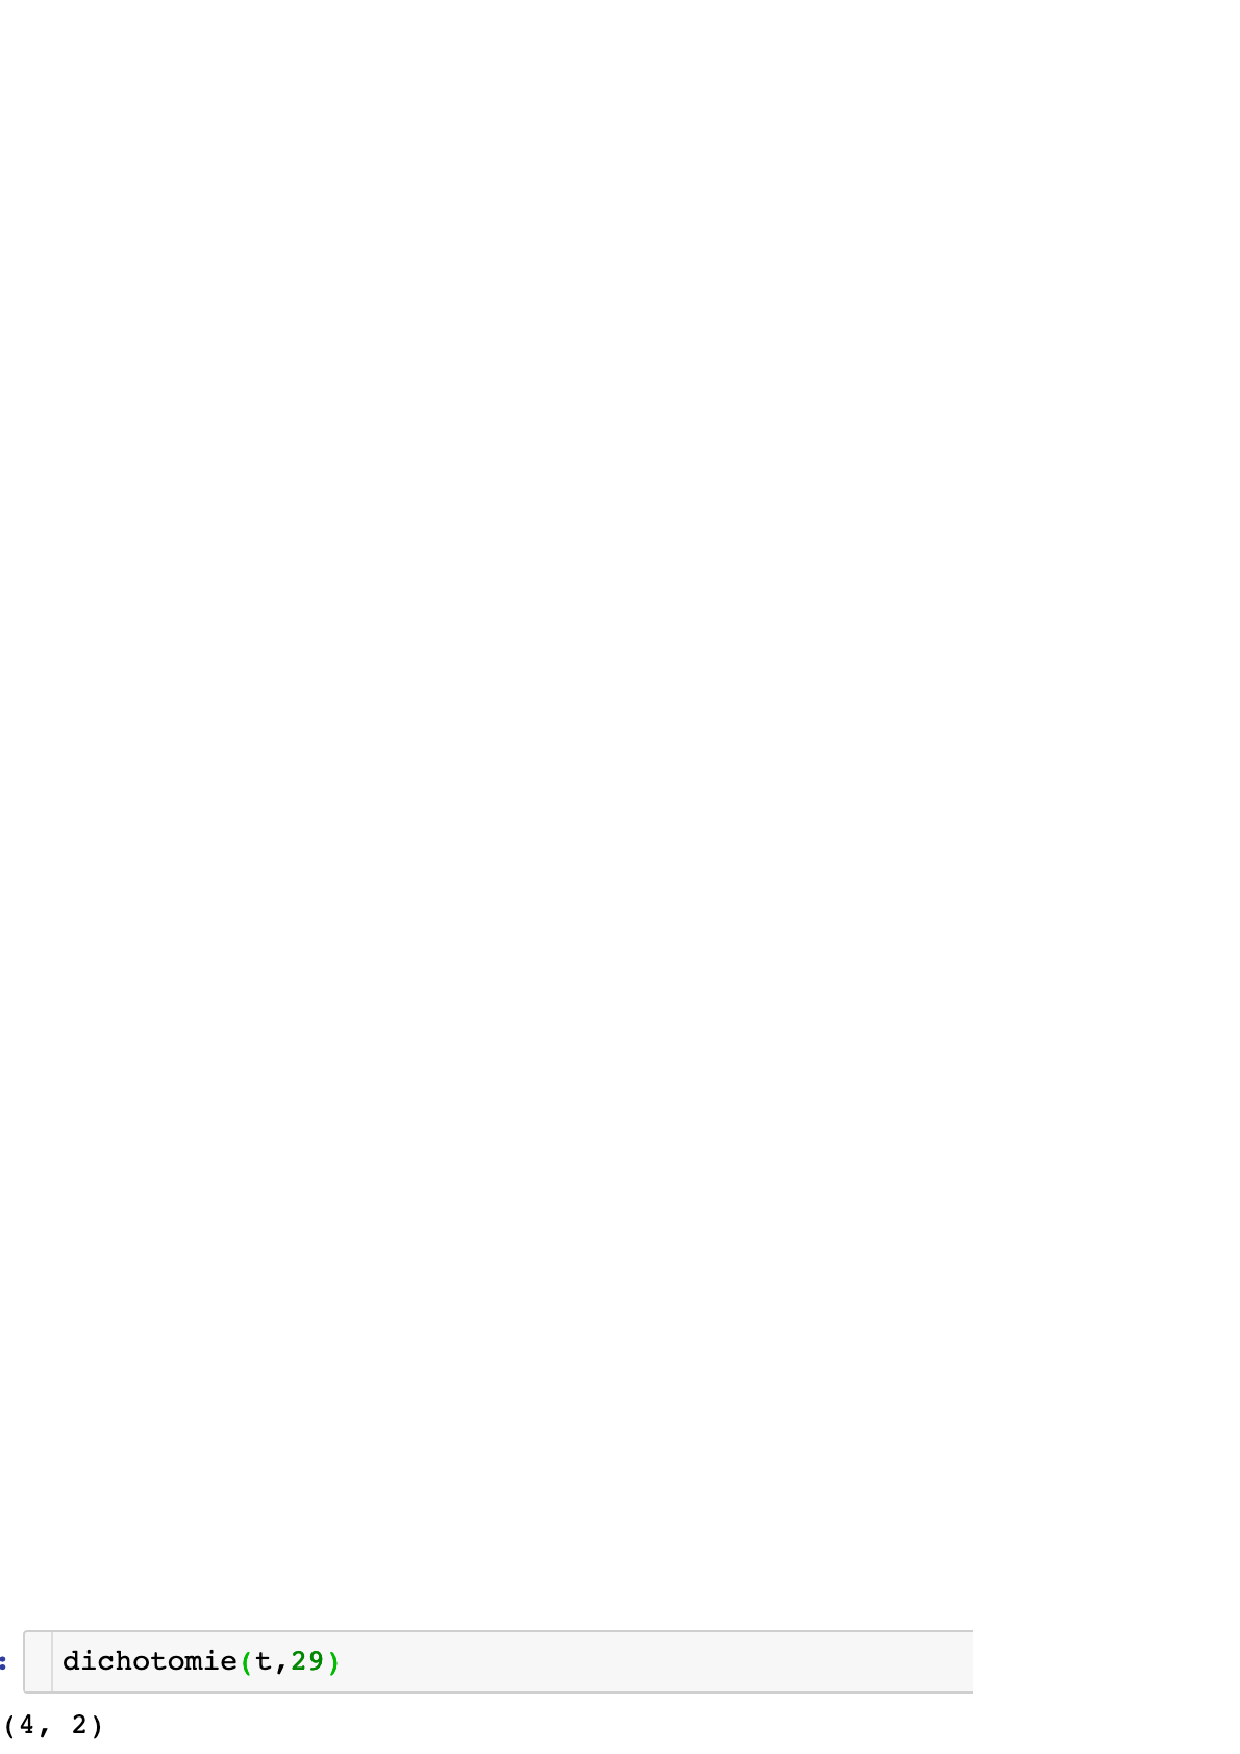
\includegraphics[scale=0.55]{../img/Ex-dicho-3-3.png}
\end{center}
\item On cherche le nombre 39 qui n'est pas dans le tableau; 5 itérations nécessaires.
\begin{center}
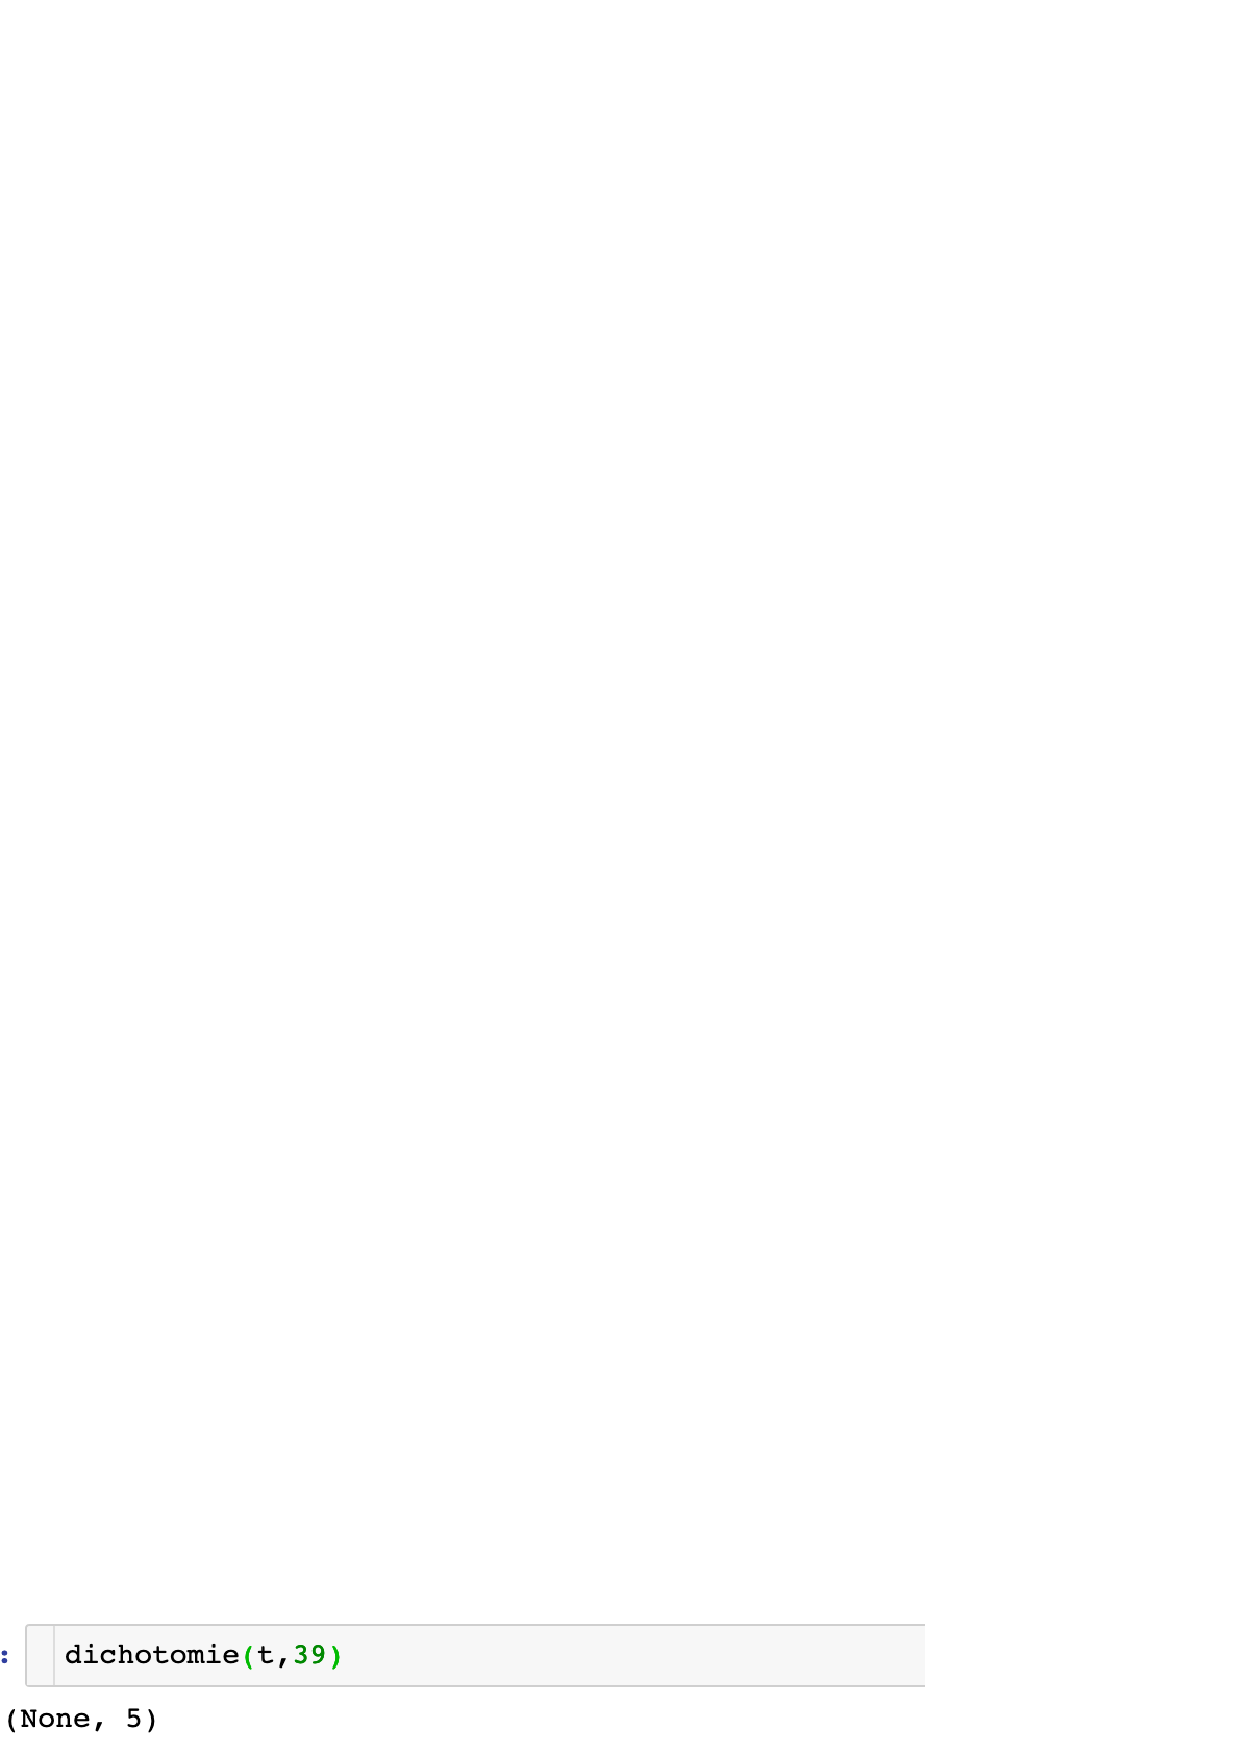
\includegraphics[scale=0.57]{../img/Ex-dicho-3-4.png}
\end{center}
\end{enumerate}
\begin{enumerate}
\item Importer le module \textbf{math} et calculer la valeur $\log_{2}(n)$:
\begin{flushleft}
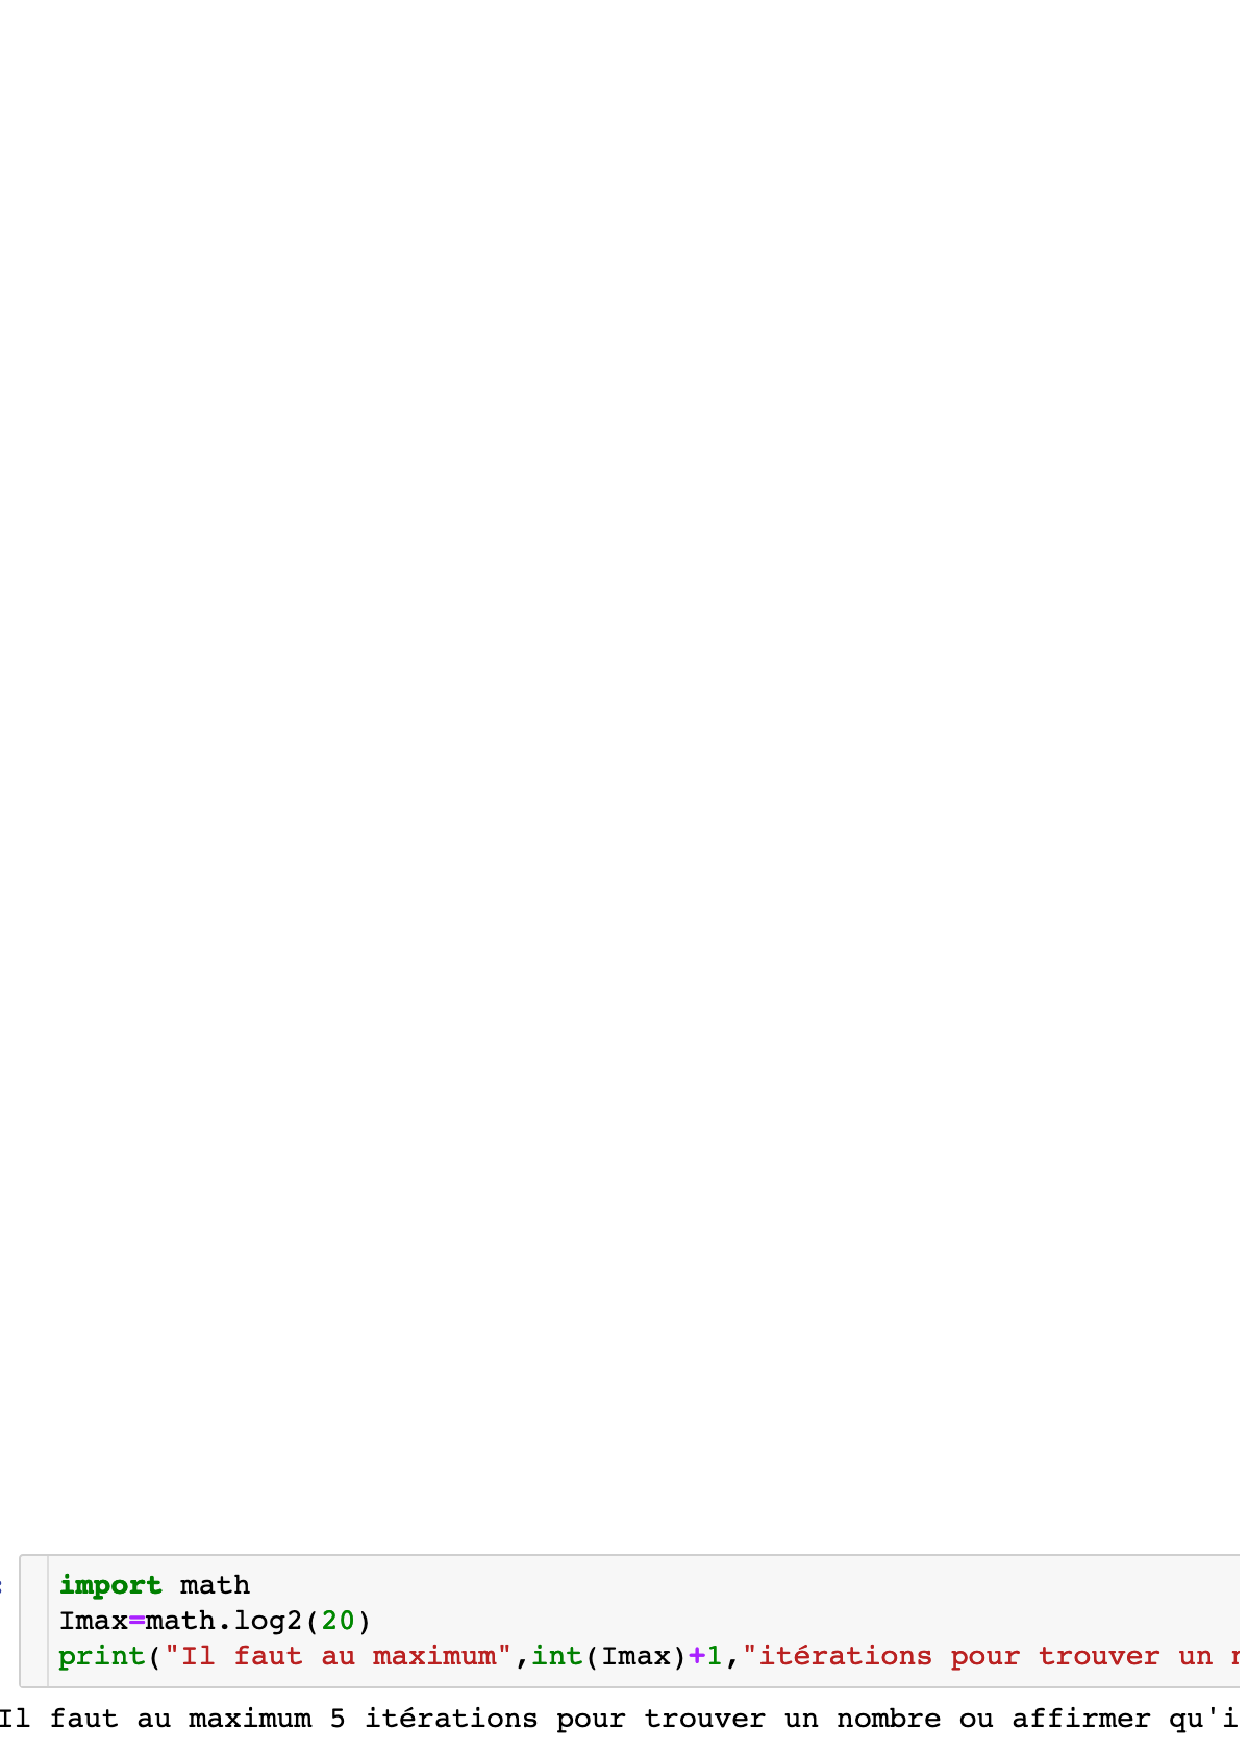
\includegraphics[scale=0.52]{../img/Ex-dicho-3-6.png}
\end{flushleft}
\item Le nombre maximal d'itérations pour un tableau de 20 valeurs est 5.
\item Boucle qui donne toutes les recherches dichotomiques pour trouver tous les nombres de votre tableau et le nombre d'itérations dans chaque cas.
On rappelle le tableau utilisé dans l'exercice:
\begin{flushleft}
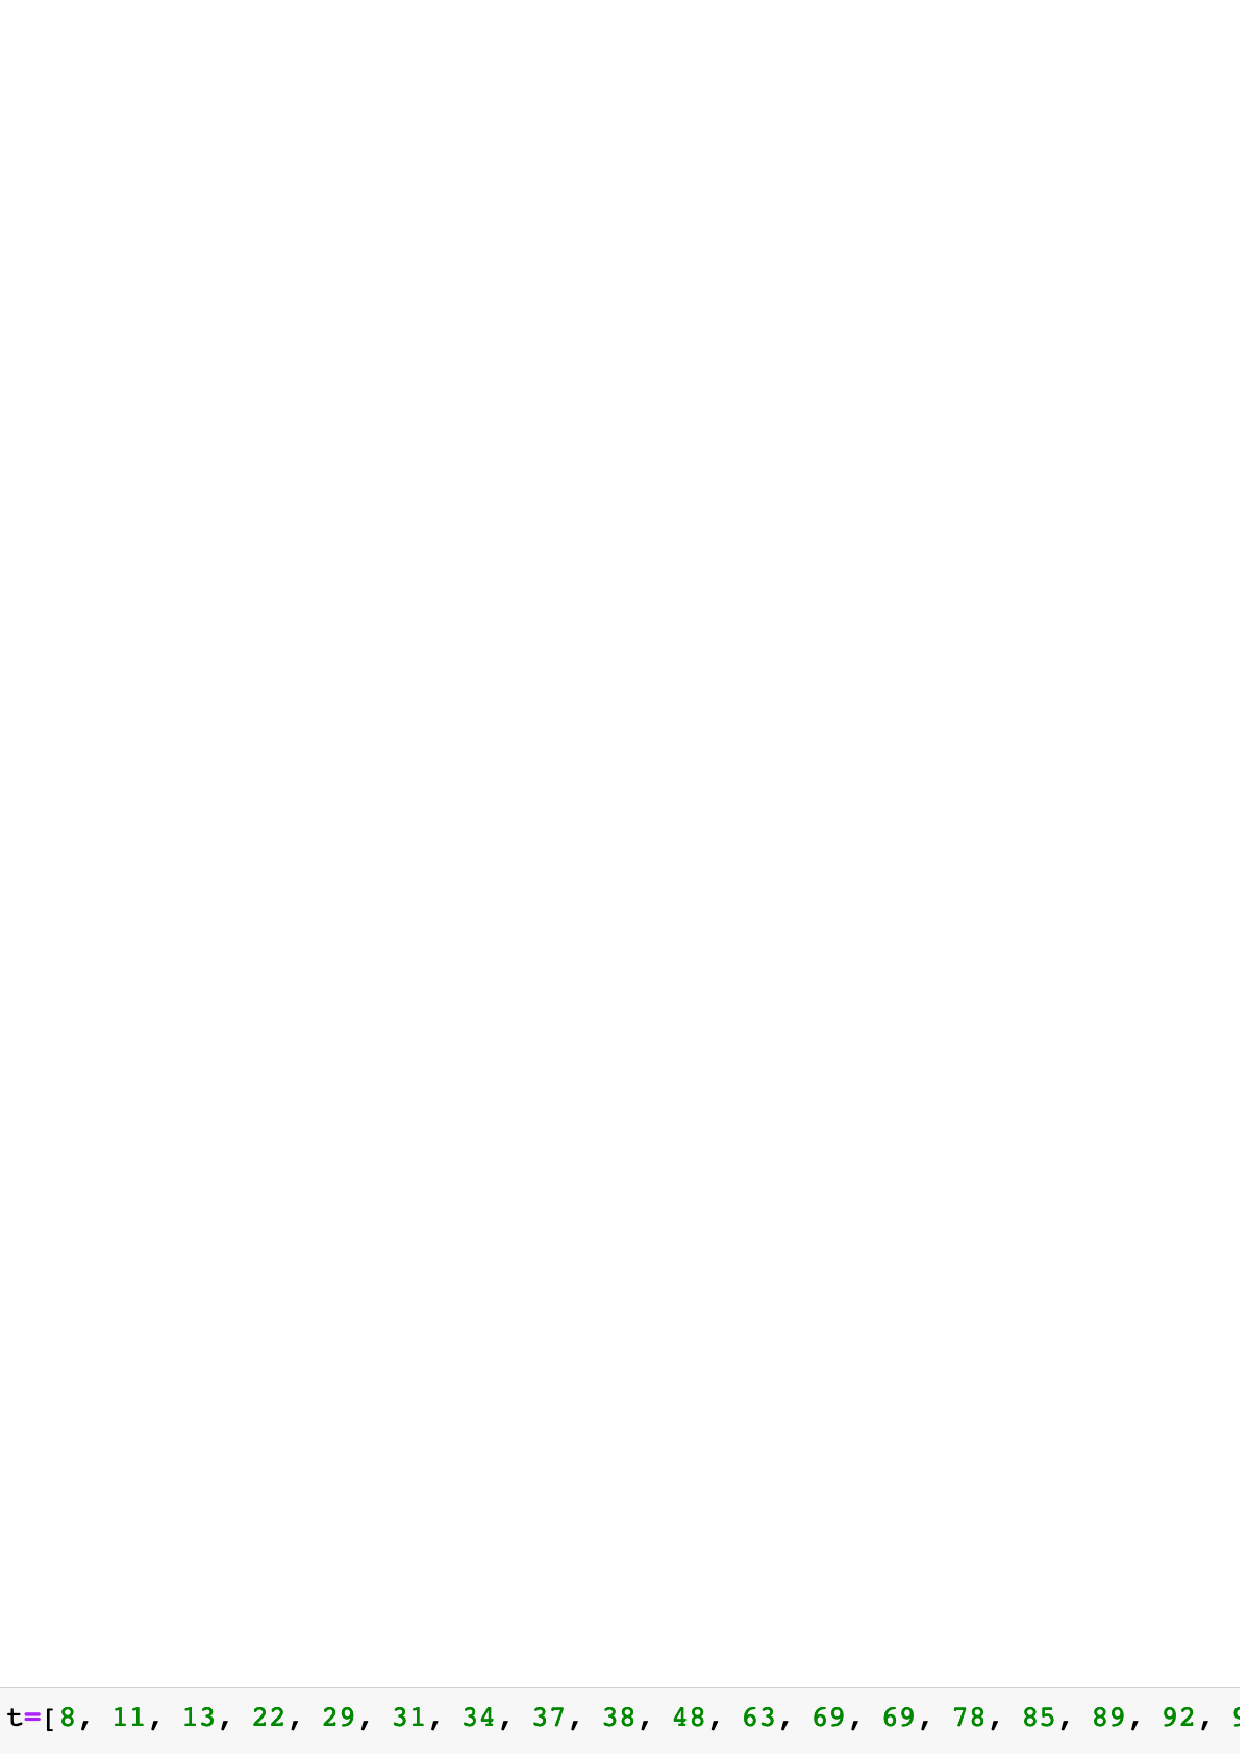
\includegraphics[scale=0.6]{../img/Ex-dicho-3-8.png}
\end{flushleft}
\begin{center}
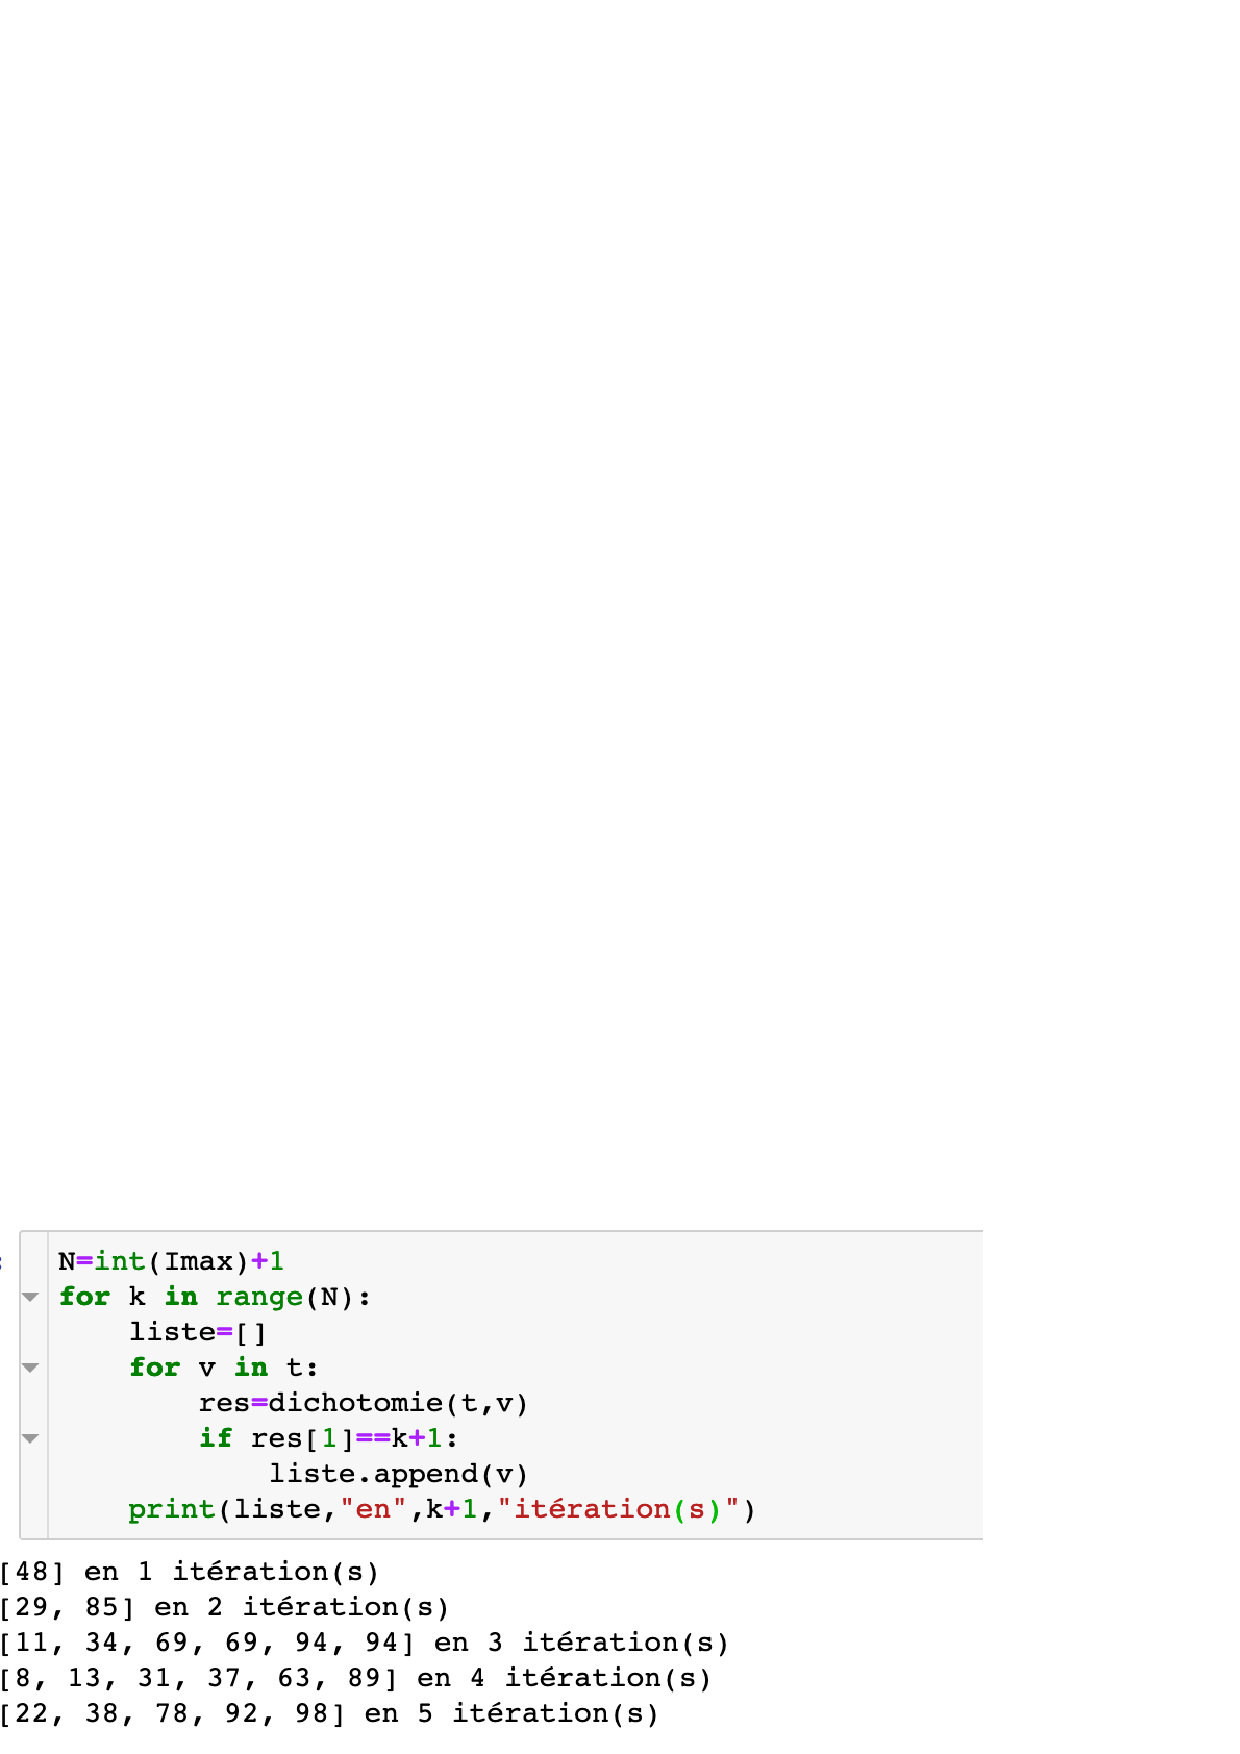
\includegraphics[scale=0.6]{../img/Ex-dicho-3-7.png}
\end{center}
\end{enumerate}
\end{enumerate}
\end{document}


